\documentclass[12pt]{article}
\usepackage[margin=1in]{geometry}
\usepackage{graphicx}
\usepackage{float}
\begin{document}
\begin{titlepage}
\title{\Huge ECS 171 Final Report}
\author{\huge Aaun Abbas\\\huge Hilal Alsibai\\\huge Christopher Chen\\\huge Miguel Covarrubias\\\huge Jesse Dyer\\\huge Pei Guo\\\huge Alex Kot\\\huge Raymond Lau\\\huge Ian Woods}
\date{}
\maketitle
\end{titlepage}

\section{Abstract}
\paragraph{}
In this project, we compared the effectiveness of several machine learning classifiers at determining forest cover types from cartographic variables. The classifiers we used were artificial neural networks, k nearest neighbors, and random forests. Our results showed that random forests more accurately predicted the correct forest cover type than any other classifier. 
\section{Introduction}
\paragraph{}
For this project, we decided to use the $Forest CoverType$ dataset from UCI's machine learning repository \cite{bache13}. Determining forest cover type from purely cartographic variables is important in situations where it is unfeasible or impossible to obtain cover type data through empirical methods. Thus, being able to accurately estimate the cover type of an area is of great interest to forest scientists \cite{blackard00, ross04}.  At the same time, the dataset provides a large amount of well structured data (581012 samples with 54 attributes) upon which different machine learning techniques can be tested and compared, making it an attractive dataset for computer scientists \cite{gama03,oza01,giannella,furnkranz,obradovic,klami}. To give an idea of how the data looks, we present some figures that show the class distribution of the data, as well as a pairwise comparison of the features.

\begin{figure}[H]
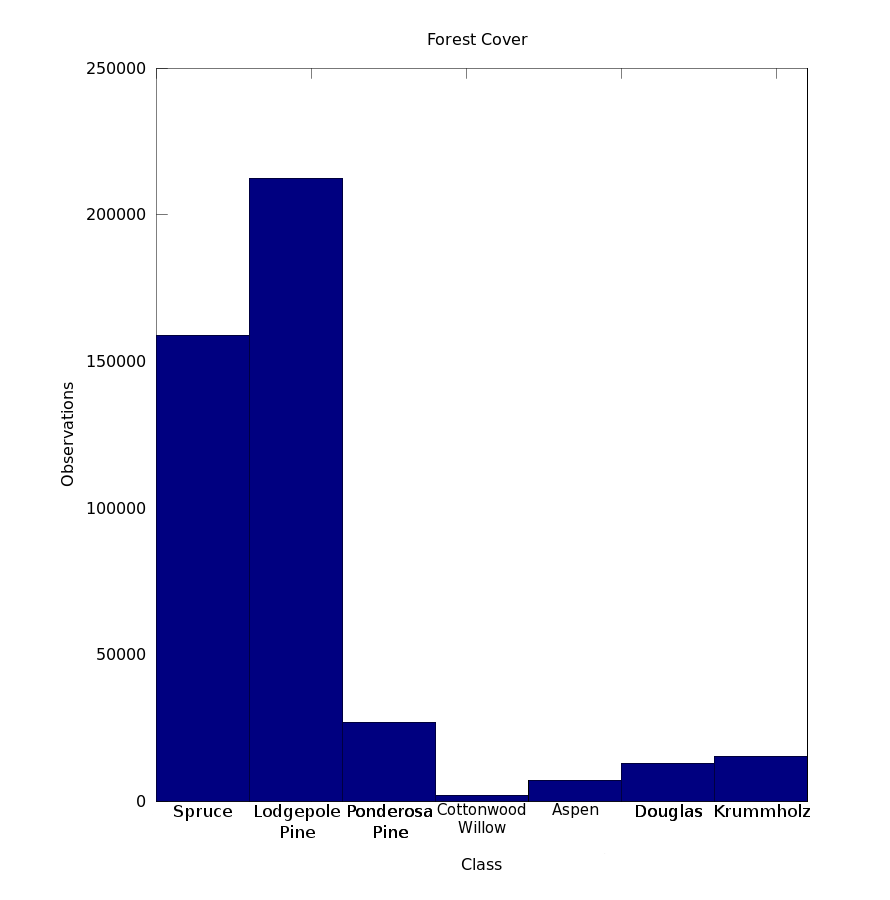
\includegraphics[width=\linewidth]{images/description.png} 
\caption{Histogram of class distribution. Note the heavy bias towards Spruce and Lodgepole Pine.}
\end{figure}

\begin{figure}[H]
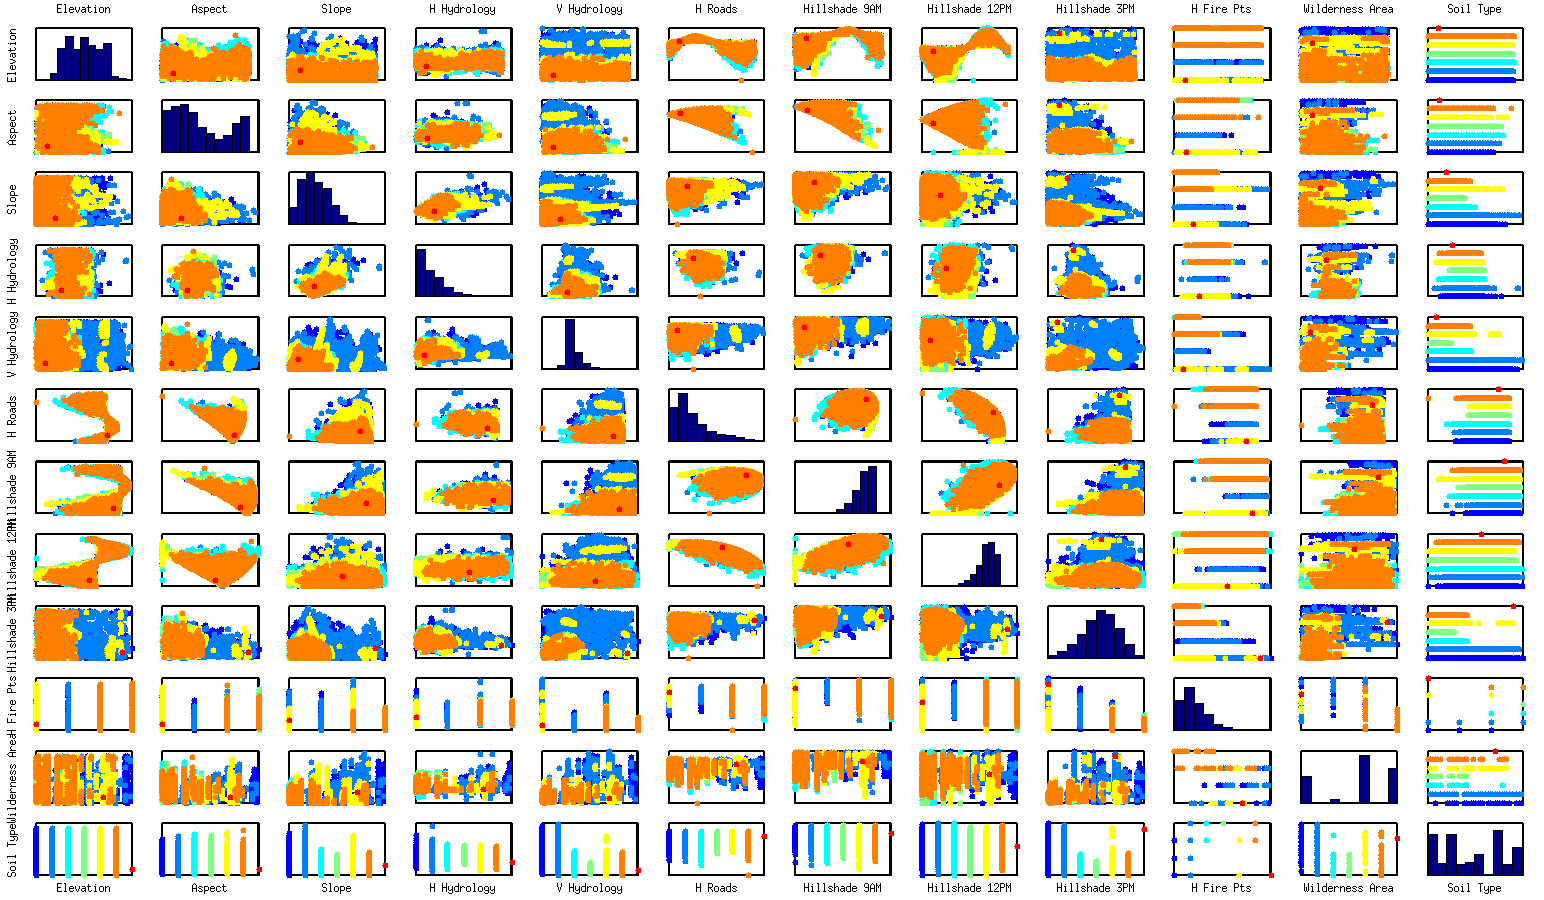
\includegraphics[width=\linewidth]{images/featureScatterPlotMatrixHD.png}
\caption{Pairwise comparison matrix of features. You may need to zoom in to see details.}
\end{figure}

\par
Research on this particular dataset has compared Gaussian discriminant analysis with artificial neural networks (ANNs).  Discriminant analysis achieved $58\%$ classification accuracy and the ANN achieved $70\%$ classification accuracy \cite{blackard00}. Blackard and Dean did not use cross validation when evaluating their classifiers, and when building their classifiers, they did not use advanced techniques such as feature selection or regularization. In this project, we improved upon their methods and provided more accurate metrics to evaluate these methods.

\section{Methods}
\paragraph{}
We used three different classifiers to determine forest cover type: artificial neural networks, k nearest neighbors, and random forests. The data contained 54 cartographic features from 581012 different 30 by 30 meter plots, along with the cover type for each plot which was determined from US Forest Service (USFS) Region 2 Resource Information System (RIS) data. Within these 54 features, 4 were boolean categorical variables describing the wilderness area, and 40 were boolean categorical variables describing the soil type. We merged the wilderness and soil type features, normalized the data, and then ran our classifiers.
\\
\begin{figure}[H]
\caption{A diagram of how we ran our classifiers.}
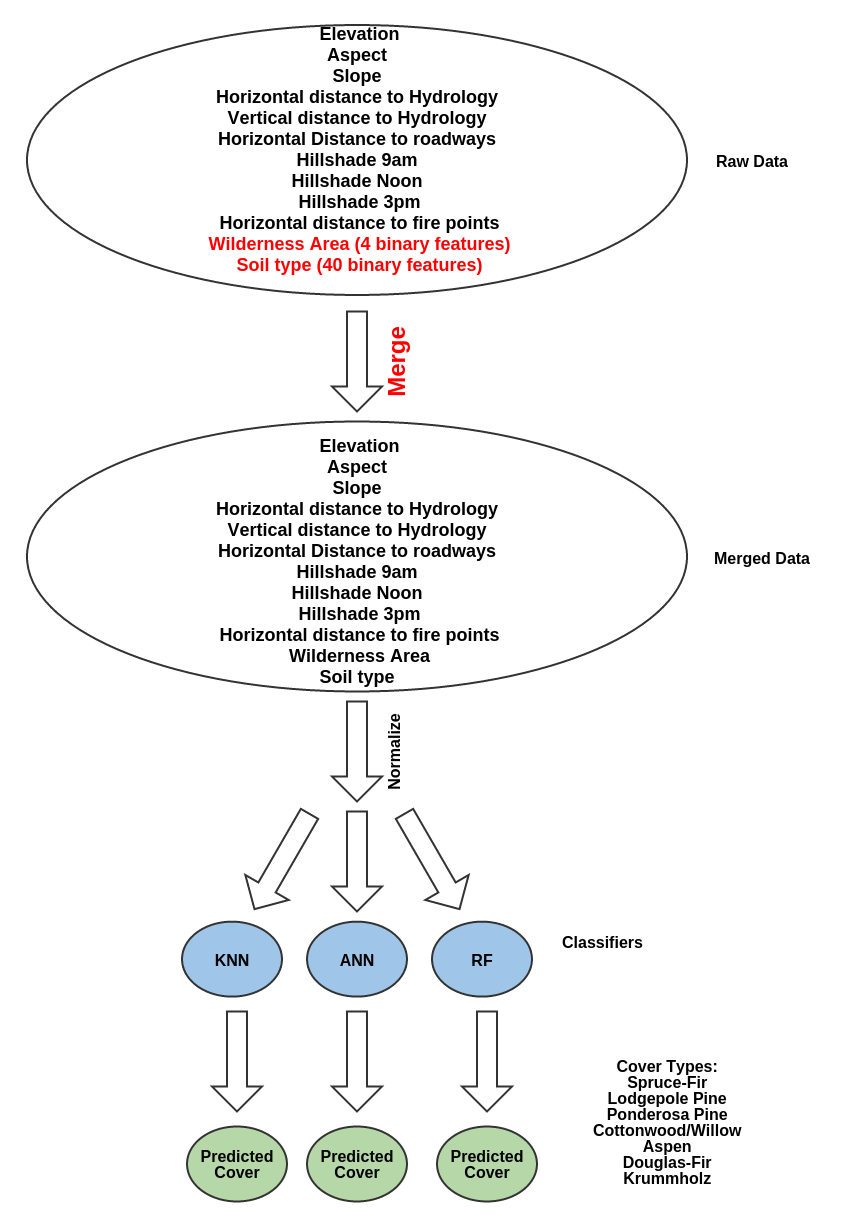
\includegraphics[width=\linewidth]{images/flow.png}
\end{figure}


\subsection{Artificial Neural Networks}
\paragraph{}
We used a deep learning toolbox in Octave to implement a feed forward back propagation ANN with L2 regularization and multiple activation functions \cite{rbp12}.  ANNs with one hidden layer and two hidden layers were evaluated with 10-fold cross validation and the misclassification rate was used as the error. The settings were: learning rate = 1.5, L2 penalty = 0.0001, number epochs = 50. We selected the ANN with the lowest misclassification rate as our classifier and used it to create both ROC curves and PR curves.  We created confusion matrices for each output node by iterating through threshold values.  From this we plotted the ROC and PR curves.  Finally, we took the predicted output for all our data through 10-fold crossvalidation and created a multiclass confusion matrix that details how classes were misclassified.

\subsection{k Nearest Neighbors}
\paragraph{}
The $k$-Nearest Neighbors (KNN) Algorithm involves classifying a given sample as a particular type, given the type of the $k$ closest samples to it, as determined by some distance function \cite{matlabpage}. Our initial approach was to use a standard Euclidean distance function, defined as follows \cite{sayad}:
\begin{center}
$\sqrt{\sum\limits_{k = 1}^n (x_{jk} - x_{ik})^2}$
\end{center}
\par
We decided to begin with this naive approach to isolate failure points (essentially, if something were to work incorrectly, we could rule out the distance function as failure point). We debated creating a distance function tailored to the dataset by hand, or by simply trying many different possible distance functions. However, we decided to generate a distance function with the largest-margin nearest neighbors algorithm (more precisely, we generated a transformation matrix that was used to transform the data, and still used the Euclidean distance). Choosing the right value for $k$ was also critical to the performance of the algorithm, so we decided to test a wide range of $k$ values in order to determine what would work best.

\par
LMNN (Largest Margin Nearest Neighbors) is a variant of KNN that can be implemented in two ways. One method is to learn a Mahalanobis distance function, which measures the distance (in standard deviations) from the center of a cluster of similarly typed samples. Another method, and the method our implementation used, is to learn a transformation matrix that, when applied to the dataset, yields higher correct classification rates \cite{huyen12}. It learns this matrix by iteratively applying small perturbations to the transformation matrix with the goal of maintaining a large distance between "impostors" (close neighbors that are of the wrong type) and the perimeters that surround groups of similarly-typed neighbors. LMNN is very helpful because it saves us the trouble of testing many different distance functions \cite{weinberger}, or trying to derive a distance function by hand for each particular dataset.
    
\subsection{Random Forests}
\paragraph{}
For random forests, we used Liaw and Wiener's R port \cite{liaw02} of Breiman's random forest algorithm \cite{breiman01}. The algorithm takes several parameters which control its speed and performance, so we used empirical analysis to determine optimal values for these parameters. The first of these was $mtry$, which controls the number of variables that are sampled at each split when building the decision trees. 7 was determined to be the optimal value, as increasing the value past 7 caused almost no change in error, but consumed far more system resources. The other parameter was $ntree$ which controls the number of trees to be generated in the forest. For the same reasons as $mtry$, 40 was found to be the optimal value.
\par
To determine error, we used the OOB (out of bag) error \cite{breiman96}. We used this estimate because it is automatically generated by the algorithm while it runs, and because cross validation is not required when using OOB error, due to the way it is computed \cite{breiman01, breiman96}, which saved us computation time. It has also been shown to be close to an optimal estimate of the generalization error\cite{breiman96}.

\section{Results}
To compare the performance of the different classifiers we used ROC and PR curves, along with the AUC. To generate ROC and PR curves for our classifiers, we used a 7-way one versus all approach (as opposed to generating ROC and PR surfaces), as generating multiclass ROC and PR curves is  computationally intensive \cite{lan07}, quite complex to implement, and generally difficult to do. This means that we split the response vector into 7 boolean response vectors and generated curves for each binary classifier trained with those vectors.

\subsection{ANN Results}
We found that the optimized tanh activation function outperformed the sigmoid function.  ANNs with one hidden layer had decreasing error until there were about 30 hidden nodes.  The one hidden layer structure did not achieve an accuracy higher than $79\%$. ANNs with two hidden layers did slightly better with the best achieving $80.3\%$ accuracy.
\\
\begin{figure}[H]
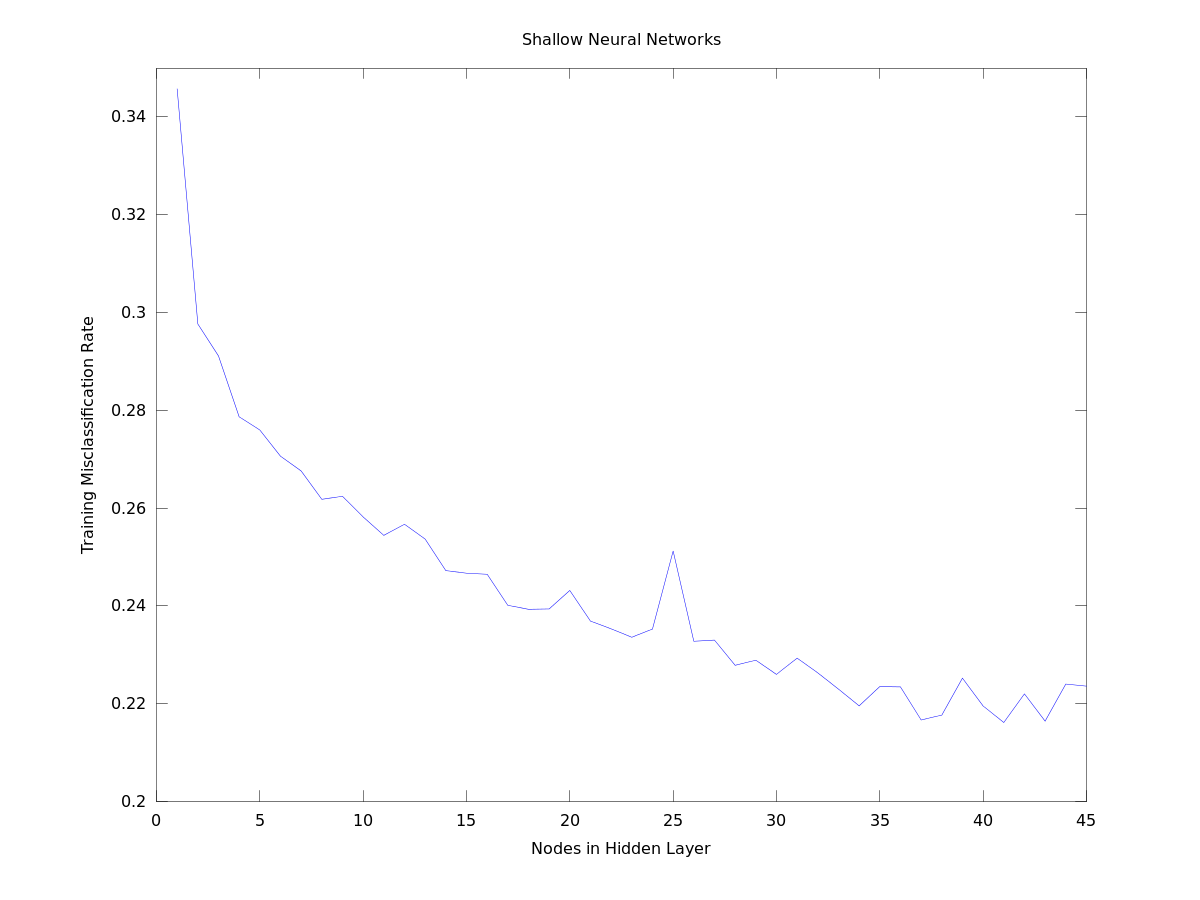
\includegraphics[width=\linewidth]{images/shallow.png}
\caption{A graph of error vs. number of nodes in the hidden layer (one hidden layer).}
\end{figure}

\begin{figure}[H]
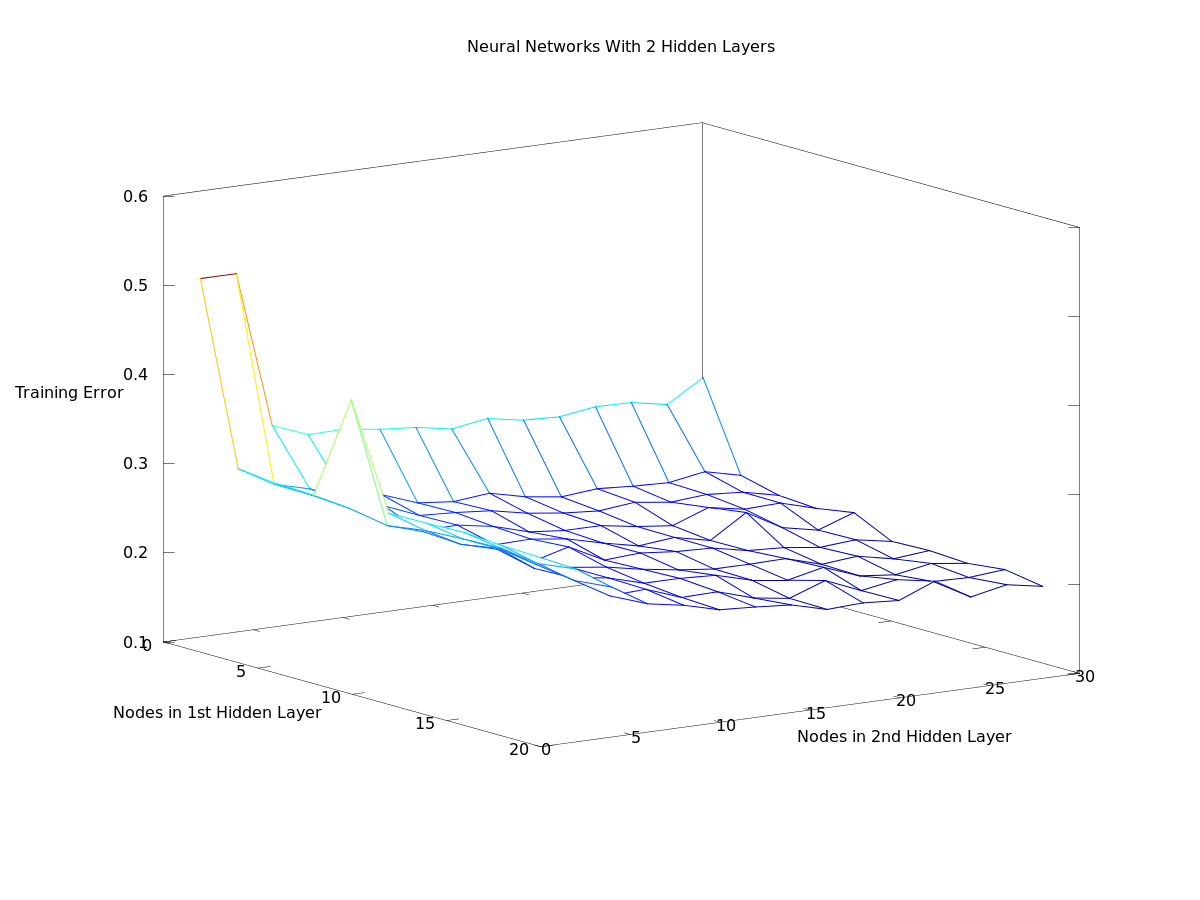
\includegraphics[width=\linewidth]{images/deep4.png}
\caption{A graph of error vs. number of nodes in the hidden layer (two hidden layers).}
\end{figure}

\begin{figure}[H]
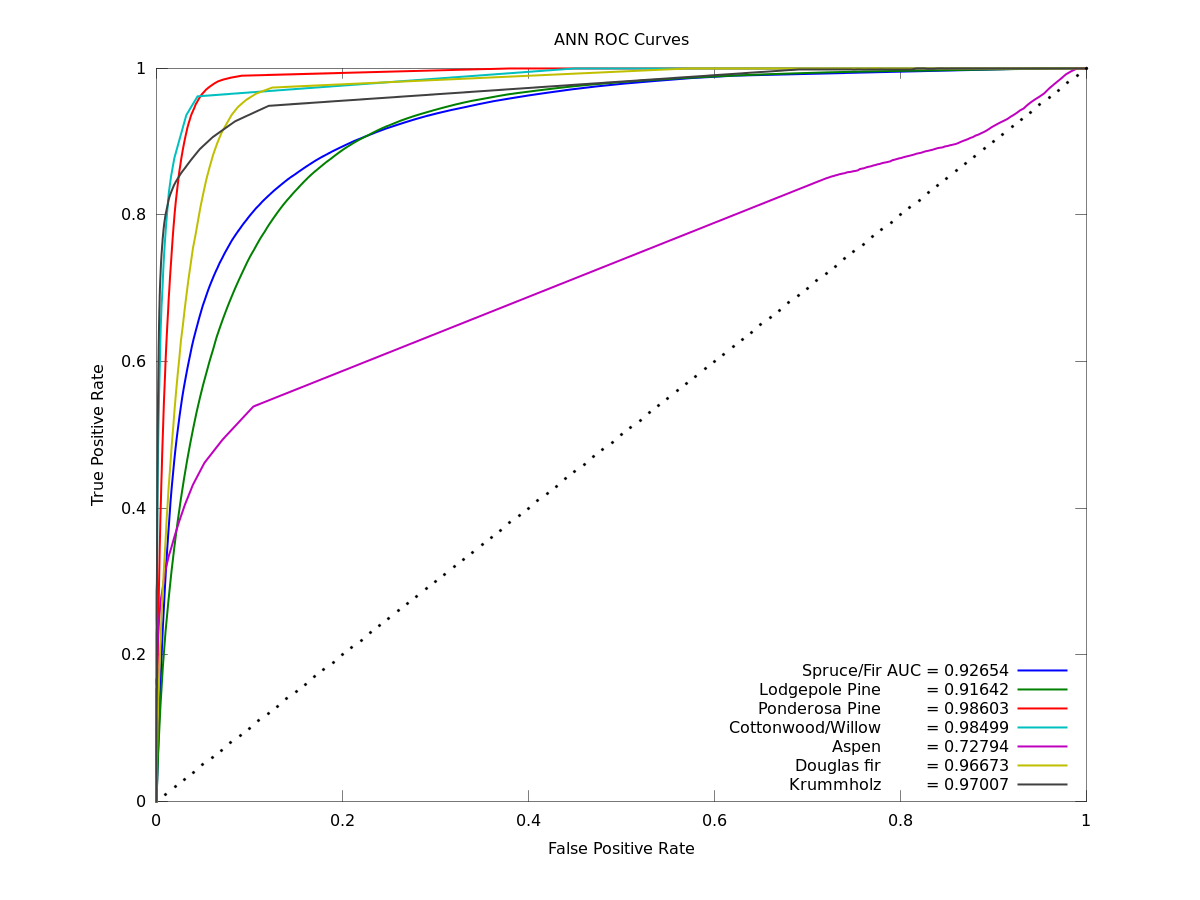
\includegraphics[width=\linewidth]{images/ROC_comp.png}
\caption{ROC curves for each class, with the AUC for each curve.}
\end{figure}

\begin{figure}[H]
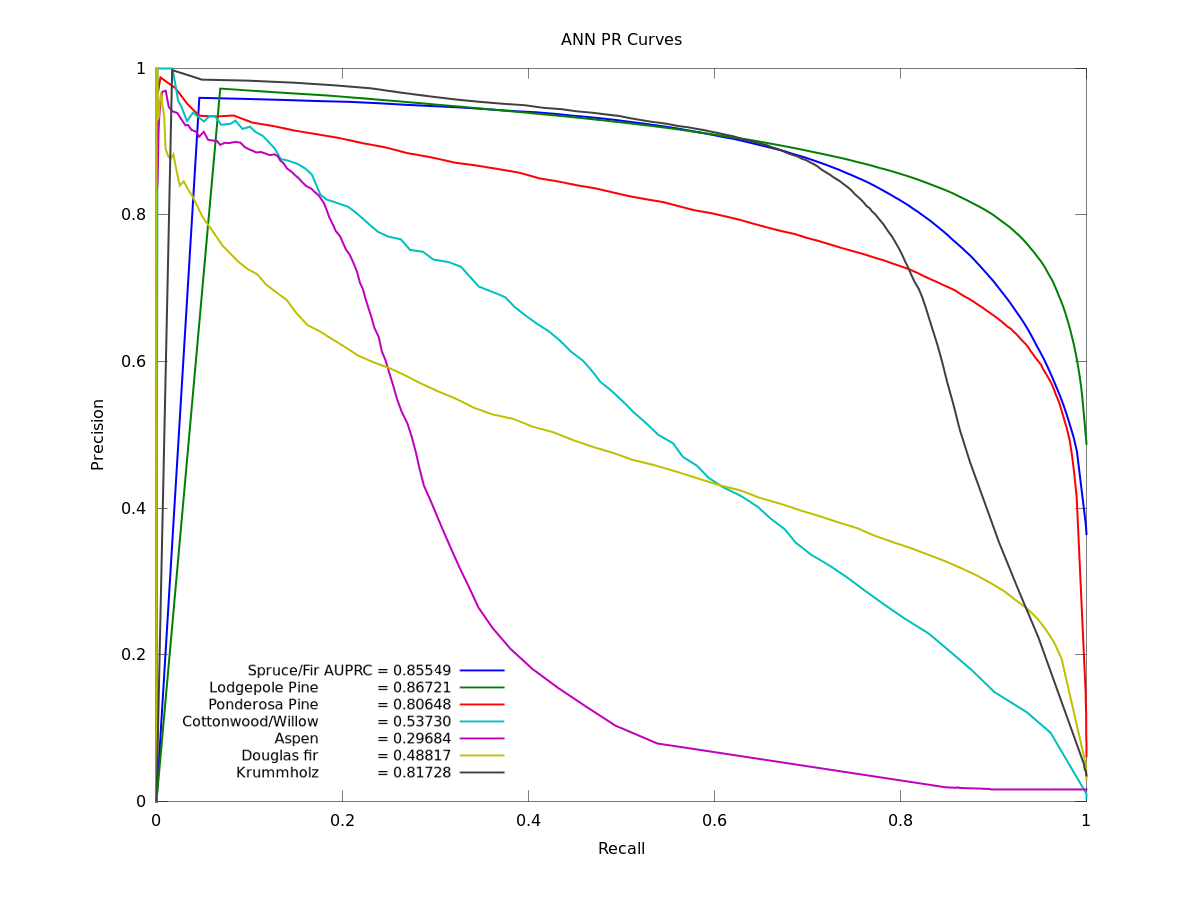
\includegraphics[width=\linewidth]{images/PR_comp.png} 
\caption{PR curves for each class, with the AUC for each curve.}
\end{figure}

The multiclass confusion matrix revealed that there was a lot of misclassificaiton between Spruce and Lodgepole pine.  Cottonwood/Willow, Aspen, and Douglas-Fir were all misclassified the majority of the time.
\begin{center}
\begin{tabular}{|c | c| c| c| c| c |c| c|}
\hline
 & Observed& Observed& Observed& Observed& Observed& Observed& Observed \\ \hline
True Class & Sp.-Fir & L. Pine & P. Pine & C./Willow & Aspen & D.-Fir & Krum \\ \hline
Sp.-Fir & \textbf{166919} & 42605 & 16 & 3 & 47 & 34 & 2216 \\ \hline
L. Pine & 28706 & \textbf{250128} & 2821 & 8 & 310 & 996 & 330 \\ \hline
P. Pine & 22 & 3140 &  \textbf{30817} & 196 & 0 & 1579 & 0 \\ \hline
C./W. & 0 & 11 & 1671 &  \textbf{863} & 0 & 202 & 0 \\ \hline
Asp. & 471 & 7176 & 288 & 0 &  \textbf{1529} & 29 & 0 \\ \hline
D.-Fir & 124 & 4303 & 8558 & 110 & 1 &  \textbf{4271} & 0 \\ \hline
Krum. & 5031 & 518 & 0 & 0 & 0 & 0 &  \textbf{14961} \\ \hline
\end{tabular}
\end{center}

\subsection{KNN Results}



\begin{figure}[H]
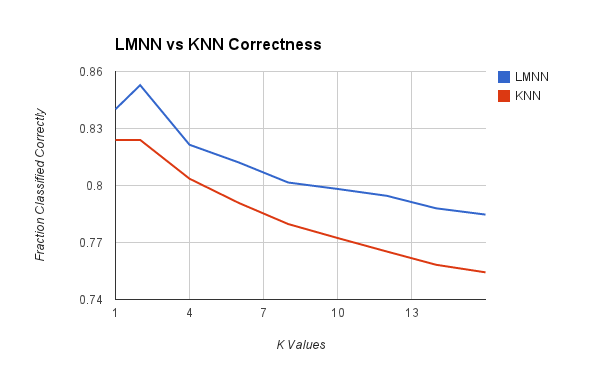
\includegraphics[width=\linewidth]{images/knnvslmnn.png}
\caption{Graph of accuracy vs. K values.}
\end{figure}
\paragraph{}
LMNN was able to boost the correct classification percentage across all values of k. On average, we saw 2.46\% better classification rates. Using LMNN, we came up with the following ROC and PR curves.
    \begin{figure}[H]
    \begin{minipage}[b]{\linewidth}
    \centering
    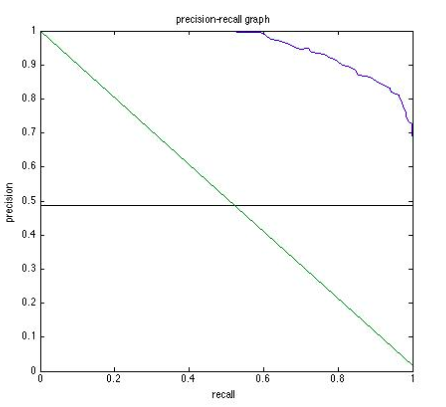
\includegraphics[width=\linewidth]{images/AspenPRCurve.png}
    \caption{PR Curve for class Aspen}
    \label{fig:chapter001_dist_001}
    \end{minipage}
    \end{figure}
    \hspace{0.5cm}
    \begin{figure}[H]
    \begin{minipage}[b]{\linewidth}
    \centering
    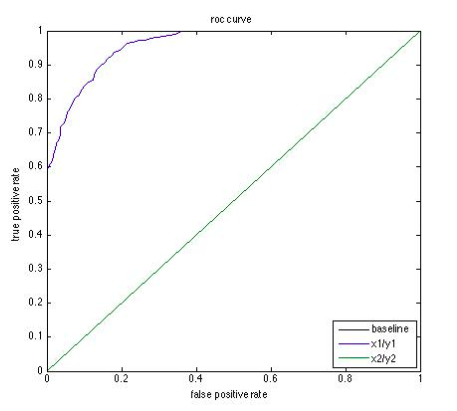
\includegraphics[width=\linewidth]{images/AspenROCCurve.png}
    \caption{ROC Curve for class Aspen}
    \label{fig:chapter001_reward_001}
    \end{minipage}
    \end{figure}
     
    \begin{figure}[H]
    \begin{minipage}[b]{\linewidth}
    \centering
    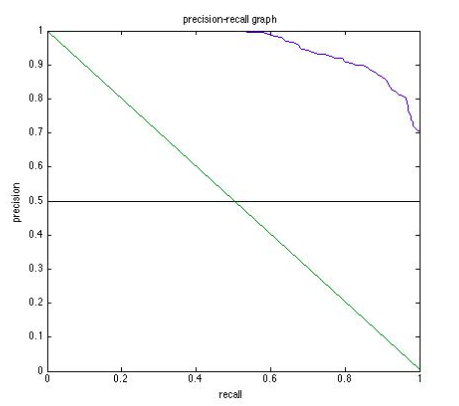
\includegraphics[width=\linewidth]{images/CottonwoodPRCurve.png}
    \caption{PR Curve for class Cottonwood}
    \label{fig:chapter001_dist_001}
    \end{minipage}
    \hspace{0.5cm}
    \end{figure}
    
    \begin{figure}[H]
    \begin{minipage}[b]{\linewidth}
    \centering
    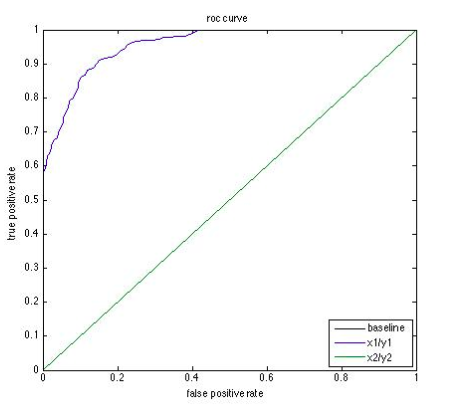
\includegraphics[width=\linewidth]{images/CottonwoodROCCurve.png}
    \caption{ROC Curve for class Cottonwood}
    \label{fig:chapter001_reward_001}
    \end{minipage}
    \end{figure}
     
    \begin{figure}[H]
    \begin{minipage}[b]{\linewidth}
    \centering
    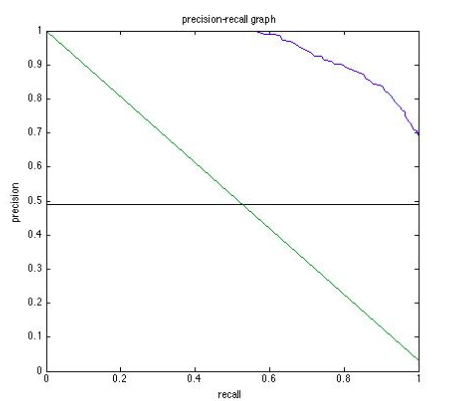
\includegraphics[width=\linewidth]{images/DouglasFirPRCurve.png}
    \caption{PR Curve for class Douglas Fir}
    \label{fig:chapter001_dist_001}
    \end{minipage}
    \hspace{0.5cm}
    \end{figure}
    \begin{figure}[H]
    \begin{minipage}[b]{\linewidth}
    \centering
    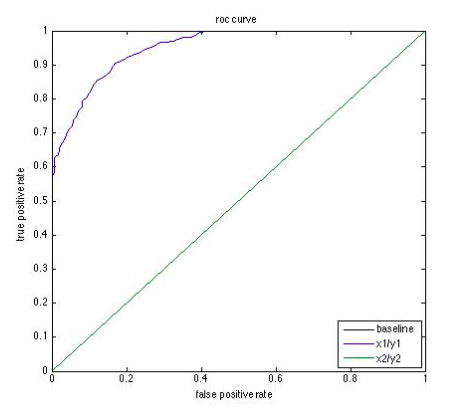
\includegraphics[width=\linewidth]{images/DouglasFirROCCurve.png}
    \caption{ROC Curve for class Douglas Fir}
    \label{fig:chapter001_reward_001}
    \end{minipage}
    \end{figure}
     
    \begin{figure}[H]
    \begin{minipage}[b]{\linewidth}
    \centering
    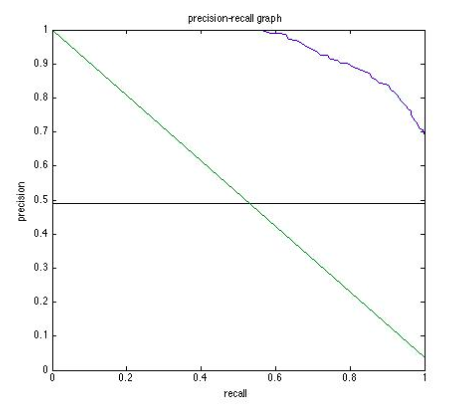
\includegraphics[width=\linewidth]{images/KrummholzPRCurve.png}
    \caption{PR Curve for class Krummholz}
    \label{fig:chapter001_dist_001}
    \end{minipage}
    \hspace{0.5cm}
    \end{figure}
    \begin{figure}[H]
    \begin{minipage}[b]{\linewidth}
    \centering
    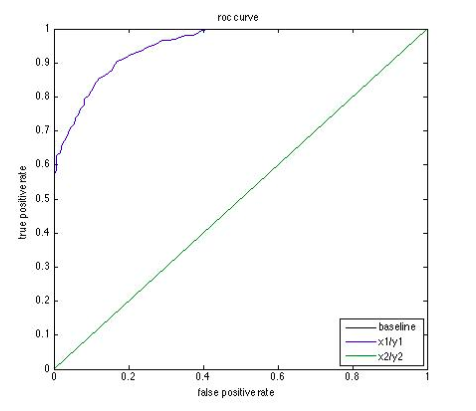
\includegraphics[width=\linewidth]{images/KrummholzROCCurve.png}
    \caption{ROC Curve for class Krummholz}
    \label{fig:chapter001_reward_001}
    \end{minipage}
    \end{figure}
     
    \begin{figure}[H]
    \begin{minipage}[b]{\linewidth}
    \centering
    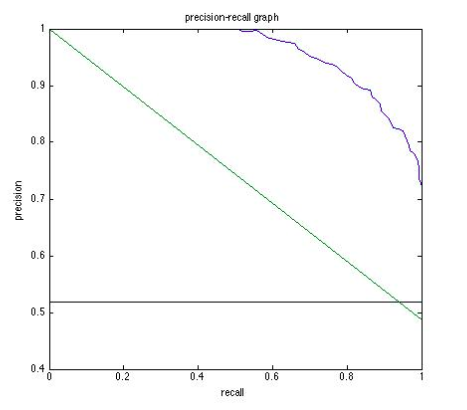
\includegraphics[width=\linewidth]{images/LodgepolePinePRCurve.png}
    \caption{PR Curve for class Lodgepole Pine}
    \label{fig:chapter001_dist_001}
    \end{minipage}
	\end{figure} 
    \hspace{0.5cm}
    \begin{figure}[H]
    \begin{minipage}[b]{\linewidth}
    \centering
    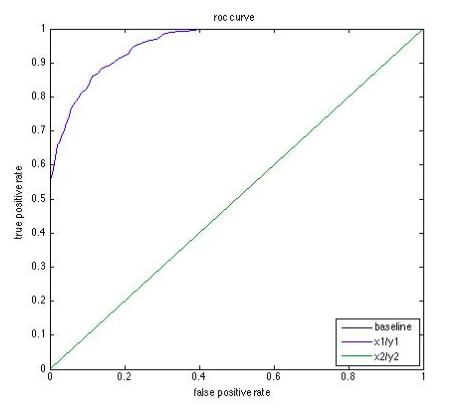
\includegraphics[width=\linewidth]{images/LodgepolePineROCCurve.png}
    \caption{ROC Curve for class Lodgepole Pine}
    \label{fig:chapter001_reward_001}
    \end{minipage}
    \end{figure}
     
    \begin{figure}[H]
    \begin{minipage}[b]{\linewidth}
    \centering
    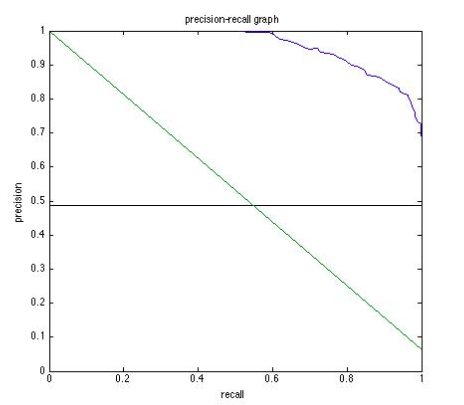
\includegraphics[width=\linewidth]{images/PonderosaPinePRCurve.png}
    \caption{PR Curve for class Ponderosa Pine}
    \label{fig:chapter001_dist_001}
    \end{minipage}
    \hspace{0.5cm}
    \end{figure}
    \begin{figure}[H]
    \begin{minipage}[b]{\linewidth}
    \centering
    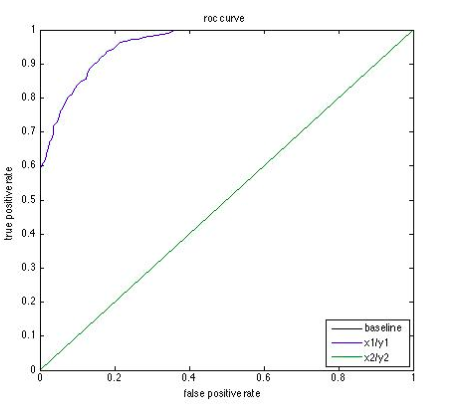
\includegraphics[width=\linewidth]{images/PonderosaPineROCCurve.png}
    \caption{ROC Curve for class Ponderosa Pine}
    \label{fig:chapter001_reward_001}
    \end{minipage}
    \end{figure}
     
    \begin{figure}[H]
    \begin{minipage}[b]{\linewidth}
    \centering
    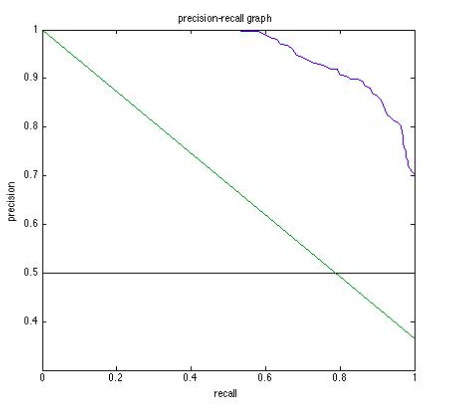
\includegraphics[width=\linewidth]{images/SpruceFirPRCurve.png}
    \caption{PR Curve for class Spruce Fir}
    \label{fig:chapter001_dist_001}
    \end{minipage}
    \hspace{0.5cm}
    \end{figure}
    \begin{figure}[H]
    \begin{minipage}[b]{\linewidth}
    \centering
    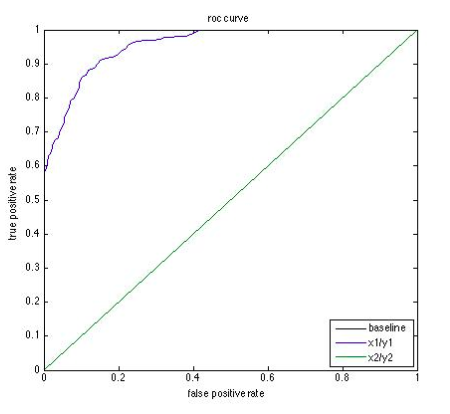
\includegraphics[width=\linewidth]{images/SpruceFirROCCurve.png}
    \caption{ROC Curve for class Spruce Fir}
    \label{fig:chapter001_reward_001}
    \end{minipage}
    \end{figure}
    
     \begin{figure}[H]
     \begin{center}
     \begin{tabular}{ l | r}
       \hline
       Cover Type & AUC \\ \hline
     
       Aspen & .892 \\ \hline
       Cottonwood & .877 \\ \hline
       Douglas Fir & .885 \\ \hline
       Krummholz & .888 \\ \hline
       Lodgepole Pine & .891 \\ \hline
       Ponderosa Pine & .883 \\ \hline
       Spruce Fir & .873 \\ \hline
     \end{tabular}
    \end{center}
    \caption{AUC for each class.}
     \end{figure}
    
    
\subsection{RF Results}
We used the ROCR library \cite{ROCR} to generate ROC and PR curves for random forests.

\begin{figure}[H]
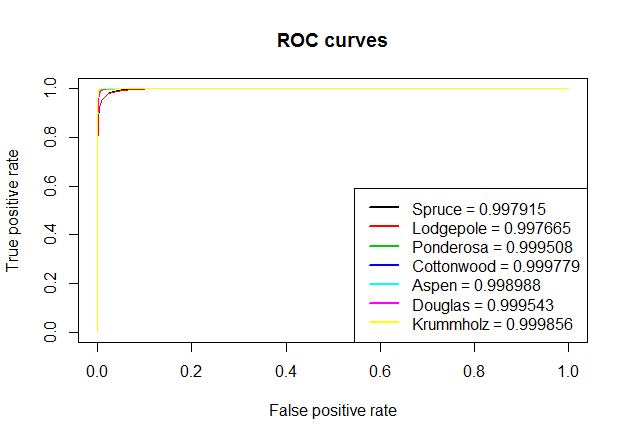
\includegraphics[width=\linewidth]{images/RFROC.png}
\caption{ROC curves for each class, with the AUC for each curve.}
\end{figure}

\begin{figure}[H]
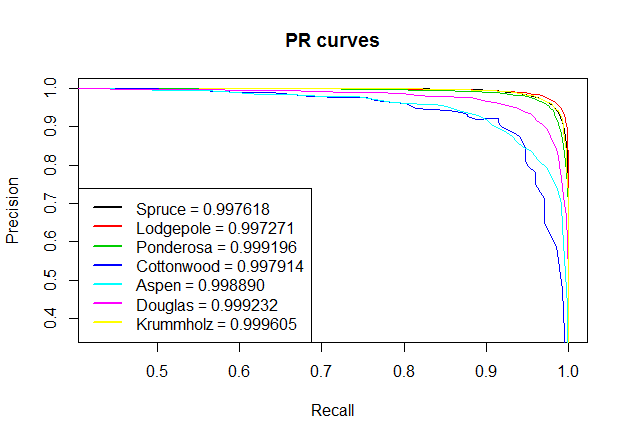
\includegraphics[width=\linewidth]{images/RFPR.png}
\caption{PR curves for each class, with the AUC for each curve.}
\end{figure}


\section{Discussion}
When weighting the importance of the AUC of a class by its representation in the data set, we get the following values for the average AUC:

\begin{figure}[H]
     \begin{center}
     \begin{tabular}{ l | r}
       \hline
       Classifier & Average AUC \\ \hline
     
       ANN & 0.92503 \\ \hline
       KNN & 0.88328 \\ \hline
       RF & 0.99803 \\ \hline
     \end{tabular}
    \end{center}
    \caption{Average AUC for each classifier.}
     \end{figure}
     
We're not quite sure why one classifier performed better or worse than another, but it could have to do with the bias present in the data. For example, ANNs had trouble correctly classifying underrepresented classes, such as Aspen. Regardless of the reasons why though, random forests outperformed ANN and KNN by 7.9\% and 13.0\% respectively, making it the clear winner.

\section{Conclusion}
In this project we used 3 different classifiers to predict forest cover type based on cartographic variables: artificial neural networks, k nearest neighbors, and random forests. We determined that random forests outperformed the other 2 classifiers. In the future, we may try to examine the performance of these classifiers on other datasets and then compare those results to those given here, or we may use different classifiers on the cover type dataset to see if we can improve our classification accuracy.

\section{Contributions}
\paragraph{}

Hilal Alsibai wrote ANN code and generated the feature comparison matrix. Alex Kot generated the ANN figures and tables, worked on the introduction, and worked on the ANN related writing. Pei Guo worked on ANN feature selection and worked on the ANN related writing.
\par
Jesse Dyer wrote / gathered most of the code for the LMNN and KNN implementations. Ian Woods generated figures, ran computations, and wrote the report. Miguel Covarrubias ran computations and generated all ROC and PR curves.
\par
Aaun Abbas and Raymond Lau wrote all of the code that was related to random forests. Christopher Chen wrote all parts of the report that were related to random forests, as well as some of the more general parts of the report. He also organized the team and took care of general logistics.

\pagebreak
\begin{thebibliography}{}
\bibitem{blackard00}
Blackard, Jock A. and Denis J. Dean. 2000. "Comparative Accuracies of Artificial Neural Networks and Discriminant Analysis in Predicting Forest Cover Types from Cartographic Variables." Computers and Electronics in Agriculture 24(3):131-151.

\bibitem{gama03}
Joao Gama and Ricardo Rocha and Pedro Medas. Accurate decision trees for mining high-speed data streams. KDD. 2003.

\bibitem{oza01}
Nikunj C. Oza and Stuart J. Russell. Experimental comparisons of online and batch versions of bagging and boosting. KDD. 2001.

\bibitem{giannella}
Chris Giannella and Bassem Sayrafi. An Information Theoretic Histogram for Single Dimensional Selectivity Estimation. Department of Computer Science, Indiana University Bloomington.

\bibitem{furnkranz}
Johannes Furnkranz. Round Robin Rule Learning. Austrian Research Institute for Artificial Intelligence.

\bibitem{obradovic}
Zoran Obradovic and Slobodan Vucetic. Challenges in Scientific Data Mining: Heterogeneous, Biased, and Large Samples. Center for Information Science and Technology Temple University.

\bibitem{klami}
Arto Klami and Samuel Kaski and Ty n ohjaaja and Janne Sinkkonen. HELSINKI UNIVERSITY OF TECHNOLOGY Department of Engineering Physics and Mathematics Arto Klami Regularized Discriminative Clustering. Regularized Discriminative Clustering.

\bibitem{liaw02}
A. Liaw and M. Wiener (2002). Classification and Regression by randomForest. R News 2(3), 18--22.

\bibitem{breiman01}
Leo Breiman. Random forests. Machine learning 45 (1), 5-32. 2001.

\bibitem{breiman96}
Breiman, Leo. Out-of-bag estimation. Technical report, Statistics Department, University of California Berkeley, Berkeley CA 94708, 1996b. 33, 34, 1996.

\bibitem{bache13}
Bache, K. \& Lichman, M. (2013). UCI Machine Learning Repository [http://archive.ics.uci.edu/ml]. Irvine, CA: University of California, School of Information and Computer Science.

\bibitem{ross04}
Ross Meentemeyer, David Rizzo, Walter Mark, Elizabeth Lotz, Mapping the risk of establishment and spread of sudden oak death in California, Forest Ecology and Management, Volume 200, Issues 1–3, 25 October 2004, Pages 195-214, ISSN 0378-1127, http://dx.doi.org/10.1016/j.foreco.2004.06.021.
(http://www.sciencedirect.com/science/article/pii/S0378112704004463)

\bibitem{rbp12}
R. B. Palm. Prediction as a candidate for learning deep hierarchical models of data. 2012.

\bibitem{lan07}
Landgrebe TCW, Duin RPW. Approximating the multiclass ROC by pairwise analysis. 2007. Pattern Recognition LEtters 28:1747-58.

\bibitem{huyen12}
    Do, Huyen, et al. A metric learning perspective of SVM: on the relation of LMNN and SVM.

    \bibitem{matlabpage}
    http://www.mathworks.com/help/stats/knnsearch.html
    
    \bibitem{sayad}
    Dr Saed Sayad. K Nearest Neighbors, 2010, http://chem-eng.utoronto.ca/~datamining/Presentations/KNN.pdf
    
    \bibitem{weinberger}
    Weinberger, Kilian Q and Saul, Lawrence K. Distance Metric Learning for Large Margin
Nearest Neighbor Classification.


\bibitem{ROCR}
Tobias Sing, Oliver Sander, Niko Beerenwinkel, Thomas Lengauer. ROCR: visualizing classifier performance in R. Bioinformatics 21(20):3940-3941 (2005).  

\end{thebibliography}
\end{document}